\documentclass[11pt,article,oneside]{memoir}

\usepackage{kjh-njb}
\usepackage{fixltx2e}
\usepackage{longtable}
\usepackage{pdflscape}
\usepackage[stable]{footmisc}
\usepackage{comment}
\usepackage{tabularx}
\usepackage{geometry}
\usepackage{rotating}
\usepackage{mathspec}
\usepackage[flushleft]{threeparttable}
\usepackage{xunicode}
\usepackage[american]{babel}
\usepackage[babel,autostyle]{csquotes}
\usepackage[authordate,sorting=nyt,backend=biber,maxcitenames=2]{biblatex-chicago}
\addbibresource{/Users/School/Dropbox/Writing/Manuscripts/bib/complete.bib} 
\DeclareFieldFormat[article]{title}{\mkbibquote{#1}}
\DeclareFieldFormat[book]{title}{\mkbibemph{#1}\isdot} % for books
\DeclareFieldFormat{booktitle}{\mkbibemph{#1}} % for edited volumes
\setmainfont[Mapping=tex-text]{Minion Pro}
%\setmainfont[ItalicFont=TisaOT-Ita,Mapping=tex-text]{Tisa OT}
\setsansfont[Mapping=tex-text]{Proxima Nova}
\setmonofont[Mapping=tex-text]{Inconsolata}
\setmathsfont(Digits)[Mapping=tex-text,Numbers=Lining]{Lyon Text}
\setmathfont(Latin)[Mapping=tex-text]{Lyon Text}
\setmathfont(Greek)[Mapping=tex-text]{Minion Pro}



\date{\today}
\begin{document} 
\fontsize{11}{15}\selectfont

\title{\bigskip \bigskip Embedded Altruism 2: Bootstrap Boogaloo}
 
\author{\small Nick Bloom\vspace{0.05in} \newline\small\emph{Duke University}}

%\author{Nick Bloom (Duke University)}



\setkeys{Gin}{width=1\textwidth} 	
\pagestyle{kjh}
\chapterstyle{article-4}
%\published{Incomplete Draft. Please do not cite without permission.}

\maketitle

%NOTE: I got a little carried away with the graphs, so are even more graphs at http://nickbloom.net/stats/eagraphs.html


Healy, Kieran. 2000. “Embedded Altruism: Blood Collection Regimes and the European Union's Donor Population.” \emph{American Journal of Sociology} 105(6): 1633–57.

\vspace{0.25in}

Kieran Healy's original paper investigated the role of institutionalized organizations in
the collection of blood across European countries. At the time, both scholarly and colloquial perspectives saw blood donation as a ''perfect example'' of individual altruism. Healy's article challenged this sentiment in two ways.

First, he compiled expectations from existing literature to construct a
'modal donor' as a series of demographic hypotheses. He then showed that this 'modal donor' is \emph{not} the most likely individual to donate blood across European countries.

Second, he demonstrated the institutional effects on blood donation by interacting individual-level characteristics with different collection
regimes. He finds both variation in the modal donor profile by
collection regime, and significant effects of the collection regimes
themselves.

In sum, Healy fails to find evidence for a singular 'modal donor', or evidence that certain individual-level traits universally predispose an individual to donate blood. Instead, Healy finds evidence that institutional and organizational contexts matter a great deal both on their own, and for the activation of individual-level donor traits. In other words, ''blood can be seen not so much as something that individuals donate, but as something that organizations collect'' (p. 1634).

\section{Data and Coding}\label{data-and-coding}

The data come from the Eurobarometer Survey, an annual survey of several European Union countries. In particular, the variables in Healy's analysis come from Eurobarometer 41.0, collected in 1994, which included several questions
about blood and plasma donation, as well as standard demographic
questions. The analyses include all of the Eurobarometer countries
except for Finland, whose respondents were missing on all the blood
donation variables.

\paragraph{Dependent Variables}\label{dependent-variables}

For the pooled within-country regressions, the
dependent variable measures whether the respondent had given blood in
the last year (about 5\% of respondents had). For the multilevel regression, the dependent variable
measures whether the respondent had ever given blood (about 27\% of respondents had).

\paragraph{Independent Variables}\label{independent-variables}

As in Healy (2000), variables are coded with the 'modal donor' as the
reference. \emph{Age} is centered on 35-year-olds. \emph{Years of
Education} is centered on those with 16 years of education, roughly
college-educated individuals. \emph{Church attendance} is coded on a
five-point scale from \texttt{0} for 'never attends' to \texttt{4} for
'attends weekly'. \emph{Income} is measured on a Eurobarometer scale
from 0-12, which standardizes income across the currencies of the
various countries (12 is highest). \emph{Sex} is coded a dichotomous measure for Female.

\emph{Network} is a four-level scale measuring the number of ties a
respondent has to a blood transfusion recipient; \texttt{0} is ties to
no one, whereas \texttt{3} is ties to self, friend/family, and someone
else who has received a transfusion.

\emph{Collection Regime} is included in the multilevel regression as a
dichotomous variable for each of the regimes, according to the coding in Healy (2000).

\section{Original Methods}\label{original-methods}

Healy uses binary logit models for the within-country analysis (equation in the original article), and a mixed-effects/multilevel logit model for the between-country analysis. The equation for the multilevel logit model is as follows:

\[log \left(\frac{p_{ij}}{1-p_{ij}}\right) = \beta_{0j} + \beta_{ij} * X_{ij} + \beta_{j} * X_{j}+ \upsilon_{j} + \epsilon_{ij}\]

where $p$ is the probability of giving blood for an individual in the
sample (the lefthand side of the equation converts this probability to
log odds). $\beta_{0j}$ is a country-level random intercept with error
term $\upsilon_{j}$, $\beta_{ij}$ is a vector of individual-level
predictors for variable vector $X_{ij}$, and $\beta_{j}$ is a vector of
country-level predictors for variable vector $X_{j}$. The residual individual term is $\epsilon_{ij}$.

\section{Original Results}\label{original-results}

I report tables and results from Healy (2003), which are corrected
versions of the tables in Healy (2000). In the within-country
regressions, Healy finds that men are more likely to donate than women
in every country (except Belgium, whose coefficient for Female is not
statistically significant). He also finds that individuals are almost
universally less likely to donate after age 35.

He finds little support for the influence of educational attainment and
income on recent donation. Education only significantly increases the
odds of donating blood in three of the countries (France, Norway, and
Greece), and is negative (but not significant) in five of the countries.
Income is only positive and significant in four of the countries
(Belgium, Netherlands, Denmark, and Norway), and two of those four are
significant at p\textless{}0.1. However, he finds significant effects for these two variables when changing the dependent variable to \emph{ever} giving blood.

Healy finds little support for the hypothesis that a respondent's
network of transfusion recipients increases that respondent's odds of
donating, with statistically significant, positive coefficients in only
three countries. Finally, he finds that, due to the organizational structure of the Red Cross, religious attendance is
statistically significant in two of the countries with Red Cross
collection regimes (and nonsignificant in all others).

The intercept terms of the pooled within-country regression show that blood banking countries exhibit the widest variation in donor rates - whereas the intercepts for Red Cross and National Systems are tightly clustered, the Banking Systems intercepts exhibit much more variance. Finally, the multilevel model reveals both the significant influence of collection regime on an individual's propensity donate, as well as the shifting modal donor between collection regimes.


\section{Replication}\label{replication}

My replications are presented in Table~\ref{tab:logits1} and Table~\ref{tab:mlm1}. Thanks to a coding memo generously supplied by Healy himself, I was able to produce near-identical results to those he found. The only differences in obtained results were due to the estimation method. Whereas Healy used \texttt{glmmPQL}, a Quasi-Likelihood approximation for his multilevel estimation (in fairness, the best method available at the time), I use the more recently-developed \texttt{lme4} package in R, which estimates multilevel GLMs using Adaptive Gauss-Hermite quadrature estimation of the 
maximum likelihood. This difference in estimation resulted in discrepancy of some coefficients due to rounding differences at the fourth decimal place - coefficient differences are, at most, 0.001.

A second difference between Healy's original tables and my replication is also an artifact of the packages I used. The packages \texttt{lme4} and \texttt{glm} now report z-statistics for glmer and glm models, rather than t-statistics. Since reporting z-scores for comparison to t-scores made little sense, I decided to report standard errors.\footnote{I know I could have \emph{computed} t-scores, but I felt like producing six pretty tables from non-standard regressions in \texttt{R} was achievement enough, and didn't want to risk something going awry.}

\paragraph{Note on Replication Results}

I compared the fit statistics of a pooled logit regression without country-level effects to the logit multilevel model, to determine whether the country-level random effects were necessary. The fit statistics for each model are in Table~\ref{tab:comp1}. Results indicate superior fit of the multilevel model across all criteria, confirming the necessity of the country-level random effect. 

\begin{table}[h]
\caption{Comparison of Single-Level and Multilevel Models \label{tab:comp1}}
\centering
\begin{tabular}{rllll}
  \toprule
 & LogLik & Deviance & AIC & BIC \\ 
\midrule
Pooled Logit (w/o CRE) & -5785.445 & 11570.890 & 11626.890 & 11829.861 \\ 
Multilevel Model (w/ CRE) & -5733.850 & 11467.700 & 11525.700 & 11735.920 \\ 
\bottomrule
\end{tabular}
\end{table}



\section{Extension}


To extend the analysis in Healy (2000), I estimate all models, both within-country and multilevel, as linear
probability models. Linear probability models (LPM) estimate binomial
outcomes using OLS. The advantage of LPMs over logit models is that the
coefficients for LPMs are the change in probability for a one-unit
change in the independent variable, whereas coefficients for logit
regressions are the change in log-odds for a one-unit change in the
independent variable.

In addition, I provide more robust estimates for coefficients from both the linear and
logit multilevel models, by presenting results from a 1000-iteration
non-parametric bootstrap of each model. Bootstrapping is a resampling method, which means that it estimates coefficients many times using many samples from the original dataset (with replacement). The result is a distribution for the coefficient, which approximates the asymptotic distribution of the coefficient's true value in the population. It therefore allows more robust and straightforward discussions of statistical significance. 

The motivation for these extensions are twofold. First, computing power
has increased dramatically in the intervening decade since the article's
initial publication, as have packages for more robust estimation. Bootstrapping now takes a matter of minutes, whereas before it look much longer.
Second, linear probability models are often touted as robust, quick
alternatives to logistic models that produce adequately accurate
results. This particular replication provided an ideal opportunity to compare the fits of both logit and LPM regressions, in order to better understand the strengths and weaknesses of each.


\subsection{Results}

\subsubsection{Pooled Within-Country Models}

The results from the LPM specifications of the pooled within-country models (Table~\ref{tab:lpms1}) are substantively identical to the logit specifications. The statistical significance of coefficients differ, but all significant coefficients in the logit specifications retain their significance in the LPM specification.


\subsubsection{Multilevel Model}

Results from the multilevel linear probability model are in Table~\ref{tab:mlm2}. Inferences from the multilevel linear probability model (MLLPM) about the influence of institutional context are the same as those those from the multilevel logit model (MLGLM). However, the institutional effects on some individual characteristics differ between the two estimation methods. The main differences are as follows:

\begin{itemize}
\item Interactions for Female * Red Cross and Female * Blood Banks are not statistically significant in the MLLPM whereas they \emph{are} significant in the MLGLM. In addition, the coefficient for Female * Donor Groups is significant in the MLLPM whereas it is not significant in the MLGLM. This is curious, given the high significance values of the Female * Blood Banks MLGLM coefficient and the Female x Donor Groups MLLPM coefficient.
\item Income * Donor Groups is not significant in the MLLPM, but is in the MLGLM.
\end{itemize}

Despite these differences, institutional contexts still significantly affect both overall propensity to donate and the modal donor profile in the MLLPM model.

\subsubsection{Bootstrapped Results}

Results from the bootstrapped MLGLM, in Table~\ref{tab:boot1}, tell much the same story as the non-bootstrapped models. Essentially, any coefficient significant at p<0.05 or higher in the MLGLM is also "statistically significant" in the bootstrapped results (doesn't contain zero in the 95\% confidence interval). These statistically significant coefficients are bold in each of the tables. The same is true for the bootstrapped MLLPM results (Table~\ref{tab:boot2}). Negative signs next to upper bounds of the 95\% confidence interval indicate nonzero values of less than 0.000. Plots of bootstrapped coefficients are in Figure~\ref{fig:boot1plot} and Figure~\ref{fig:boot2plot}.

Most importantly, all coefficients for each institutional context (Red Cross, Blood Banks, and Donor Groups) are robustly nonzero in both of the bootstrapped results. The bootstrapped linear probability model indicates institutional effects as high as a 25-30\% increase/decrease in the propensity of an individual to give based on his or her institutional context.

\subsection{Comparison of Model Fit}


\subsubsection{MLM}

Table~\ref{tab:mlmcomp} presents fit statistics for both the MLLPM and the MLGLM. The MLGLM uses one more degree of freedom than the MLLPM because of the fixed residual variance. The fit statistics indicate significantly superior model fit by the MLGLM across log likelihood, AIC, and BIC. These results indicate that the logit specification for probability ought to be preferred in this case.

To further explore the model fit, I examined the number of unexpected donors produced by each model. I defined an unexpected donor as an individual who had ever donated blood, but whom the model (either MLLPM or MLGLM) predicted as having a probability lower than 0.5. Thus, according to the model, that particular donor should \emph{not} have donated blood.

Figure~\ref{fig:countries} shows unexpected donors by model across countries, and Figure~\ref{fig:colreg} shows unexpected donors by model across collection regimes. In all cases except France, the logit specification of the model produces either the same number of or fewer unexpected donors. These results, combined with model fit statistics above, indicate a superior fit by the MLGLM.\footnote{I did a similar test with donors whose P(Donation)<0.1. The MLGLM contained 39 of these individuals, the MLLPM contained 70.}

\subsubsection{Pooled Within-Country Regression}

Table~\ref{tab:slcomp} presents fit statistics for the logit and LPM specifications of each of the pooled within-country models. In every case, the LPM provides significantly superior fit over the logit specification. This finding lends support to the use of LPMs in place of logit models. Neither model produced predicted probabilities above 0.5 for any donor, so comparisons of 'unexpected' donors wasn't possible.




\begin{table}
\centering
\newcolumntype{d}{D{.}{.}{2}}
\caption{Fit Statistics for Single-Level Models\label{tab:slcomp}} 
\begin{tabular}{l*{4}{d}}
  \toprule
\multicolumn{1}{l}{Country} & \multicolumn{1}{c}{logit BIC} & \multicolumn{1}{c}{LPM BIC} & \multicolumn{1}{c}{logit AIC} & \multicolumn{1}{c}{LPM AIC} \\ 
  \midrule
France & 585.36 & 446.13 & 552.30 & 408.35 \\ 
 Belgium & 228.01 & -136.34 & 198.12 & -170.51 \\ 
Netherlands & 530.68 & 283.54 & 497.41 & 245.51 \\ 
Germany & 794.62 & -47.26 & 756.49 & -90.83 \\ 
Italy & 321.15 & -83.32 & 289.19 & -119.85 \\ 
Luxembourg & 182.62 & -27.24 & 155.06 & -58.74 \\ 
Denmark & 616.94 & 427.82 & 583.33 & 389.42 \\ 
Ireland & 318.31 & 130.49 & 288.23 & 96.11 \\ 
GB & 383.87 & 131.22 & 352.05 & 94.86 \\ 
Greece & 484.18 & 348.21 & 451.72 & 311.12 \\ 
Spain & 332.72 & -35.03 & 300.97 & -71.31 \\ 
Portugal & 259.07 & -469.96 & 226.23 & -507.50 \\ 
Norway & 357.91 & -198.21 & 324.61 & -236.27 \\ 
   \bottomrule
\end{tabular}
\end{table}

\begin{table}
\centering
\newcolumntype{d}{D{.}{.}{3}}
\caption{Fit Statistics for Multilevel Models\label{tab:mlmcomp}} 
\begin{tabular}{l*{4}{d}}
  \hline
\multicolumn{1}{l}{Model} & \multicolumn{1}{c}{DF} & \multicolumn{1}{c}{AIC} & \multicolumn{1}{c}{BIC} & \multicolumn{1}{c}{logLik} \\ 
  \hline
GLM & 29.000 & 11525.700 & 11735.921 & -5733.850 \\ 
  LPM & 30.000 & 12053.349 & 12270.819 & -5996.675 \\ 
   \hline
\end{tabular}
\end{table}


\section{Discussion}\label{discussion}

\subsection{Substantive Results}

Overall, the original findings in Healy (2000) are robust across estimation methods. While there are some differences in specific interpretations between the MLLPM and MLGLM models, both models confirm the importance of institutional context both independently and for the salience of individual donor characteristics. The importance of institutional context is upheld in the bootstrapped confidence intervals as well.

\subsection{LPMs and GLMs}

A particularly interesting finding was the wide gap between the LPM specification of the MLLPM and the MLGLM. The BIC of the MLGLM is over 500 'points' better than the MLLPM - a clear victory for the MLGLM. However, the superior fit of all LPM specifications for the pooled within-country regressions complicates a straightforward methodological prescription.

In order to test the effect of the dependent variable on model fit, I re-ran the pooled within-country models with "ever donated" as the dependent variable. In these models, the logit specification provided superior fit across all models. 

There are two possible explanations. First, the latent probability (if I may) differs between the two dependent variables. Donating in the last year has a linear shape, while ever donating has a more logarithmic shape. Second, and more likely, the differences in model fit has to do with the proportion of "successes" in the binomial dependent variable. I'll be running a simulation to test this, and will report the results soon. Overall, this variable fit indicates that researchers ought to test \emph{both} specifications, to see which is better.



\newgeometry{margin=1in}
\begin{landscape}

\begin{table}
\fontsize{10}{12}\selectfont
\centering
\newcolumntype{d}{D{.}{.}{6}}
\begin{threeparttable}
\caption{Logistic regression on donor variable: Individual-level effects by country \label{tab:logits1}}
\def\sym#1{\ifmmode^{#1}\else\(^{#1}\)\fi}
\begin{tabularx}{8in}{X*{8}{d}}\\
\toprule
\multicolumn{1}{c}{Country} & \multicolumn{1}{c}{Intercept} & \multicolumn{1}{c}{Female} & \multicolumn{1}{c}{Age} & \multicolumn{1}{c}{Education} & \multicolumn{1}{c}{Income} & \multicolumn{1}{c}{Network} & \multicolumn{1}{c}{Attend} & \multicolumn{1}{c}{\emph{N}} \\
\midrule
\textbf{National Systems} & & & & & & & & \\
\midrule
Britain &-1.833\sym{***} &  -0.430 & -0.041\sym{***} &   0.037 & 0.013 & -0.218 & -0.002 & 696 \\
& (0.279) &  (0.306) &   (0.011) &  (0.041) & (0.045) & (0.241) & (0.138)& \\
France &-1.633\sym{***} &  -0.149 & -0.024\sym{***} &   0.134\sym{***} & 0.034 &  0.055 &  0.075 & 831 \\
& (0.223) &  (0.231) &   (0.008) &  (0.032) & (0.035) & (0.160) & (0.118)& \\
Ireland &-1.912\sym{***} &  -0.753\sym{***} & -0.032\sym{***} &  -0.004 & 0.055 &  0.107 & -0.031 & 543 \\
& (0.502) &  (0.360) &   (0.013) &  (0.083) & (0.060) & (0.272) & (0.145)& \\
\textbf{Red Cross Systems} & & & & & & & & \\
\midrule
Belgium &-2.900\sym{***} &   0.097 & -0.005 &   0.024 & 0.115\sym{*} &  0.128 &  0.103& 529 \\
& (0.483) &  (0.440) &   (0.013) &  (0.028) & (0.068) & (0.307) & (0.186)& \\
Luxembourg &-3.119\sym{***} &  -1.389\sym{***} & -0.013 &  -0.067 & 0.105 & -0.209 &  0.498\sym{***}& 379 \\
& (0.578) &  (0.578) &   (0.016) &  (0.074) & (0.078) & (0.326) & (0.219)& \\
Netherlands &-2.427\sym{***} &  -0.289 & -0.021\sym{**} &  -0.001 & 0.060\sym{*} &  0.312\sym{*} &  0.220\sym{**}& 857 \\
& (0.252) &  (0.253) &   (0.009) &  (0.032) & (0.035) & (0.184) & (0.097)& \\
Germany &-2.771\sym{***} &  -0.493\sym{**} & -0.028\sym{***} &   0.017 & 0.004 &  0.502\sym{***} &  0.095 & 1714 \\
& (0.211) &  (0.213) &   (0.007) &  (0.024) & (0.032) & (0.149) & (0.103)& \\
\textbf{Banking Systems} & & & & & & & & \\
\midrule
Denmark&-1.923\sym{***} &  -0.368 & -0.018\sym{**} &  -0.003 & 0.077\sym{**} &  0.144 &  0.074 & 898 \\
& (0.222) &  (0.234) &   (0.008) &  (0.024) & (0.033) & (0.166) & (0.130) & \\
Norway&-2.709\sym{***} &  -0.143 & -0.011 &   0.039\sym{**} & 0.125\sym{**} &  0.124 &  0.039 & 860 \\
& (0.322) &  (0.332) &   (0.011) &  (0.019) & (0.053) & (0.229) & (0.180) & \\
Italy&-2.754\sym{***} &  -1.207\sym{***} & -0.021\sym{*} &  -0.007 &-0.015 & -0.134 &  0.214 & 710 \\
& (0.483) &  (0.403) &   (0.011) &  (0.043) & (0.062) & (0.289) & (0.161) & \\
Greece &-1.476\sym{***} &  -1.863\sym{***} & -0.030\sym{***} &   0.068\sym{**} & 0.024 &  0.005 &  0.202 & 763 \\
& (0.411) &  (0.343) &   (0.008) &  (0.031) & (0.049) & (0.214) & (0.170) & \\
Spain &-2.852\sym{***} &  -0.193 & -0.017 &   0.038 & 0.020 &  0.297 &  0.117 & 689 \\
& (0.396) &  (0.343) &   (0.012) &  (0.042) & (0.056) & (0.269) & (0.135) & \\
Portugal & -3.742\sym{***} & -1.631\sym{***} & -0.004 &  -0.049 & 0.120 &  0.614 & 0.154 & 806 \\
& (0.596) & (0.491) &  (0.014) & (0.054) & (0.078) & (0.373) & (0.197) & \\
\bottomrule
\end{tabularx}
\begin{tablenotes}
\item \scriptsize{Standard Errors are given in parentheses below coefficients.}
\item \scriptsize{\sym{*} \emph{P} < 0.1}
\item \scriptsize{\sym{**} \emph{P} < 0.05}
\item \scriptsize{\sym{***} \emph{P} < 0.01}
\end{tablenotes}
\end{threeparttable}
\fontsize{10}{15}\selectfont
\end{table}

\end{landscape}
\restoregeometry

\begin{table}
\fontsize{10}{12}\selectfont
\centering
\newcolumntype{d}{D{.}{.}{6}}
\begin{threeparttable}
\caption{Mixed-effects logit model of individual- and institutional-level variables \label{tab:mlm1}}
\def\sym#1{\ifmmode^{#1}\else\(^{#1}\)\fi}
\begin{tabularx}{4.25in}{X*{4}{d}}\\
\toprule
\multicolumn{1}{l}{Variable} & \multicolumn{1}{c}{Main Effect} & \multicolumn{1}{c}{Red Cross} & \multicolumn{1}{c}{Blood Banks} & \multicolumn{1}{c}{Donor Groups}\\
\midrule
Intercept & -0.388\sym{*} & & & \\
 & (0.042) & & & \\[0.25em]
Female  & -0.430\sym{***} & -0.222\sym{*} & -0.419\sym{***} & -0.175 \\
 & (0.107) &  (0.134) & (0.126) & (0.125) \\[0.25em]
Age &  0.013\sym{***} & -0.011\sym{***} &  0.004 & -0.006 \\
&  (0.003) &  (0.004) & (0.004) & (0.004) \\[0.25em]
Education &  0.061\sym{***} & -0.029 & -0.039\sym{**} &  0.024\sym{*} \\
 & (0.017) &  (0.019) & (0.017) & (0.013) \\[0.25em]
Income  &  0.098\sym{***} & -0.059\sym{***} & -0.001 & -0.039\sym{**} \\
&  (0.017) &  (0.021) & (0.020) & (0.020) \\[0.25em]
Network &  0.158\sym{**} &  0.258\sym{***} &  0.089 &  0.045 \\
&  (0.078) &  (0.097) & (0.089) & (0.089) \\[0.25em]
Attend  &  0.017 &  0.043 & -0.031 &  0.009 \\
&  (0.046) &  (0.059) & (0.060) & (0.060) \\[0.25em]
Red Cross & -0.747\sym{***} & & & \\
  & (0.055) & & & \\ [0.25em]
Bld. Banks & -0.842\sym{***} & & & \\
  & (0.052) & & & \\ [0.25em]
Donor Grp & 0.803\sym{***} & & & \\
  & (0.050) & & & \\ [0.25em]
\bottomrule
\end{tabularx}
\begin{tablenotes}
\item \scriptsize{NOTE: Valid N=10,394. Log Likelihood = -5734.}
\item \scriptsize{Country-level random effects fitted but not shown.}
\item \scriptsize{Standard Errors are given in parentheses below coefficients.}
\item \scriptsize{\sym{*} \emph{P} < 0.1}
\item \scriptsize{\sym{**} \emph{P} < 0.05}
\item \scriptsize{\sym{***} \emph{P} < 0.01}
\item \scriptsize{Estimated using \texttt{lmer} in \texttt{R}}
\end{tablenotes}
\end{threeparttable}
\fontsize{10}{15}\selectfont
\end{table}

\newgeometry{margin=1in}
\begin{landscape}
\begin{table}
\fontsize{10}{12}\selectfont
\centering
\newcolumntype{d}{D{.}{.}{6}}
\begin{threeparttable}
\caption{Linear Probability Model of Donor Variable: Individual-level effects by country \label{tab:lpms1}}
\def\sym#1{\ifmmode^{#1}\else\(^{#1}\)\fi}
\begin{tabularx}{8in}{X*{8}{d}}\\
\toprule
\multicolumn{1}{c}{Country} & \multicolumn{1}{c}{Intercept} & \multicolumn{1}{c}{Female} & \multicolumn{1}{c}{Age} & \multicolumn{1}{c}{Education} & \multicolumn{1}{c}{Income} & \multicolumn{1}{c}{Network} & \multicolumn{1}{c}{Attend} & \multicolumn{1}{c}{\emph{N}} \\
\midrule
 \textbf{National Systems} & & & & & & & & \\
\midrule
Britain  &  0.131\sym{***}  & -0.029  &  -0.002\sym{***}  &    0.003  & -0.001  &  -0.013  &  0.001  & 696\\
 & (0.021) & (0.020) &  (0.001)  &  (0.003) & (0.003) &  (0.015) & (0.009) & \\
France  &  0.171\sym{***}  & -0.016  &  -0.002\sym{**}  &    0.015\sym{***}  &  0.002  &   0.004  &  0.008  & 831\\
 & (0.022) & (0.022) &  (0.001)  &  (0.003) & (0.003) &  (0.015) & (0.011) & \\
Ireland  &  0.127\sym{***}  & -0.050\sym{**}  &  -0.002\sym{**}  &    0.000  &  0.003  &   0.006  & -0.002  & 543\\
 & (0.037) & (0.023) &  (0.001)  &  (0.006) & (0.004) &  (0.018) & (0.011) & \\
 \textbf{Red Cross Systems} & & & & & & & & \\
\midrule
Belgium  &  0.057\sym{***}  &  0.003  &   0.000  &    0.001  &  0.005\sym{*}  &   0.005  &  0.004  & 529\\
 & (0.021) & (0.018) &  (0.001)  &  (0.002) & (0.003) &  (0.013) & (0.008) & \\
Luxembourg &       0.058\sym{*}  & -0.059\sym{*}  &  -0.001  &   -0.003  &  0.004  &  -0.010  &  0.023\sym{*}  & 379 \\
 & (0.024) & (0.023) &  (0.001)  &  (0.003) & (0.003) &  (0.015) & (0.010) & \\
Netherlands  &   0.086\sym{***}  & -0.022  &  -0.001\sym{**}  &    0.000  &  0.004  &   0.024\sym{*}  &  0.018\sym{**}  & 857\\
 & (0.019) & (0.019) &  (0.001)  &  (0.002) & (0.003) &  (0.014) & (0.008) & \\
Germany  &   0.065\sym{***}  & -0.026\sym{**}  &  -0.001\sym{***}  &    0.001  &  0.000  &   0.027\sym{***}  &  0.005  & 1714\\
 & (0.012) & (0.012) &  (0.000)  &  (0.001) & (0.002) &  (0.008) & (0.006) & \\
 \textbf{Banking Systems} & & & & & & & & \\
\midrule
Denmark  &   0.128\sym{***}  & -0.032  &  -0.001\sym{**}  &   -0.001  &  0.006\sym{**}  &   0.012\sym{**}  &  0.007  & 898\\
 & (0.021) & (0.021) &  (0.001)  &  (0.002) & (0.003) &  (0.015) & (0.011) & \\
Norway  &   0.064\sym{***}  & -0.005  &   0.000  &    0.002\sym{**}  &  0.005\sym{**}  &   0.004  &  0.002  & 860\\
 & (0.015) & (0.015) &  (0.000)  &  (0.001) & (0.002) &  (0.010) & (0.008) & \\
Italy  &   0.067\sym{***}  & -0.054\sym{***}  &  -0.001\sym{**}  &   -0.001  & -0.001  &  -0.008  &  0.010  & 710\\
 & (0.023) & (0.017) &  (0.001)  &  (0.002) & (0.003) &  (0.014) & (0.008) & \\
Greece  &   0.185\sym{***}  & -0.137\sym{***}  &  -0.002 \sym{***} &    0.005\sym{*}  &  0.001  &  -0.001  &  0.021  & 763\\
 & (0.036) & (0.023) &  (0.001)  &  (0.003) & (0.004) &  (0.017) & (0.014) & \\
Spain  &   0.059\sym{***}  & -0.011  &  -0.001  &    0.002  &  0.001  &   0.015  &  0.006  & 689\\
 & (0.020) & (0.018) &  (0.001)  &  (0.002) & (0.003) &  (0.014) & (0.007) & \\
Portugal  &   0.034\sym{**}  & -0.045\sym{***}  &   0.000  &   -0.001  &  0.003  &   0.016  &  0.005  & 806 \\
 & (0.017) & (0.013) &  (0.000)  &  (0.002) & (0.002) &  (0.010) & (0.006) & \\
 \bottomrule
\end{tabularx}
\begin{tablenotes}
\item \scriptsize{Standard Errors are given in parentheses below coefficients.}
\item \scriptsize{\sym{*} \emph{P} < 0.1}
\item \scriptsize{\sym{**} \emph{P} < 0.05}
\item \scriptsize{\sym{***} \emph{P} < 0.01}
\end{tablenotes}
\end{threeparttable}
\fontsize{10}{15}\selectfont
\end{table}
\end{landscape}
\restoregeometry

\begin{table}
\fontsize{10}{12}\selectfont
\centering
\newcolumntype{d}{D{.}{.}{6}}
\begin{threeparttable}
\caption{Mixed-effects linear probability model of individual- and institutional-level variables \label{tab:mlm2}}
\def\sym#1{\ifmmode^{#1}\else\(^{#1}\)\fi}
\begin{tabularx}{4.25in}{X*{4}{d}}\\
\toprule
\multicolumn{1}{l}{Variable} & \multicolumn{1}{c}{Main Effect} & \multicolumn{1}{c}{Red Cross} & \multicolumn{1}{c}{Blood Banks} & \multicolumn{1}{c}{Donor Groups}\\
\midrule
Intercept & 0.416\sym{***} & & & \\
 & (0.042) & & & \\[0.25em]
Female  & -0.081\sym{***} & -0.041 & -0.038 & -0.078\sym{***} \\
 & (0.021) & (0.025) & (0.023) & (0.022)\\[0.25em]
Age &  0.002\sym{***} & -0.002\sym{**} &  0.000 &  0.000 \\
 & (0.001) & (0.001) & (0.001) & (0.001)\\[0.25em]
Education &  0.014\sym{***} & -0.008\sym{**} & -0.011\sym{***} &  0.006\sym{**} \\
 & (0.003) & (0.004) & (0.003) & (0.002)\\[0.25em]
Income  &  0.018\sym{***} & -0.011\sym{***} & -0.005 & -0.003 \\
 & (0.003) & (0.004) & (0.004) & (0.004)\\[0.25em]
Network &  0.031\sym{**} &  0.048\sym{***} &  0.004 &  0.021 \\
 & (0.015) & (0.018) & (0.017) & (0.016)\\[0.25em]
Attend  &  0.003 &  0.008 & -0.005 &  0.001 \\
 & (0.009) & (0.011) & (0.011) & (0.011)\\[0.25em]
Redcross & -0.157\sym{***} & & & \\ 
  & (0.055) & & & \\ [0.25em]
Bld. Banks & -0.183\sym{***} & & & \\ 
  & (0.052) & & & \\ [0.25em]
Donor Grp & 0.172\sym{***} & & & \\ 
  & (0.050) & & & \\ [0.25em]
\bottomrule
\end{tabularx}
\begin{tablenotes}
\item \scriptsize{NOTE: Valid N=10,394. Log Likelihood = -6117.}
\item \scriptsize{Country-level random effects fitted but not shown.}
\item \scriptsize{Standard Errors are given in parentheses below coefficients.}
\item \scriptsize{\sym{*} \emph{P} < 0.1}
\item \scriptsize{\sym{**} \emph{P} < 0.05}
\item \scriptsize{\sym{***} \emph{P} < 0.01}
\item \scriptsize{Estimated using \texttt{lmer} in \texttt{R}}
\end{tablenotes}
\end{threeparttable}
\fontsize{10}{15}\selectfont
\end{table}

\begin{table}
\fontsize{10}{12}\selectfont
\centering
\newcolumntype{d}{D{.}{.}{6}}
\begin{threeparttable}
\caption{Bootstrap Results for Mixed-effects logit model \label{tab:boot1}}
\def\sym#1{\ifmmode^{#1}\else\(^{#1}\)\fi}
\begin{tabularx}{4.5in}{X*{3}{d}}\\
\toprule
\multicolumn{1}{l}{Variable} & \multicolumn{1}{c}{Coefficient} & \multicolumn{1}{c}{95\% CI Lower} & \multicolumn{1}{c}{95\% CI Upper}\\
\midrule
(Intercept) & -0.388 & -0.822 & 0.065 \\
\textbf{Female} & -0.430 & -0.644 & -0.205 \\ 
Female x Red Cross & -0.222 & -0.496 & 0.049 \\ 
\textbf{Female x Blood Banks} & -0.419 & -0.669 & -0.168 \\  
Female x Don. Grp. & -0.175 & -0.432 & 0.072 \\   
\textbf{Age} & 0.013 & 0.006 & 0.019 \\ 
\textbf{Age x Red Cross} & -0.011 & -0.020 & -0.003 \\
Age x Blood Banks & 0.004 & -0.004 & 0.011 \\
Age x Don. Grp. & -0.006 & -0.014 & 0.002 \\
\textbf{Education} & 0.061 & 0.028 & 0.094 \\ 
Education x Red Cross & -0.029 & -0.065 & 0.008 \\
\textbf{Education x Blood Banks} & -0.039 & -0.073 & -0.004 \\
Education x Don. Grp. & 0.024 & -0.002 & 0.050 \\ 
\textbf{Income} & 0.098 & 0.062 & 0.134 \\ 
\textbf{Income x Red Cross} & -0.059 & -0.104 & -0.014 \\
Income x Blood Banks & -0.001 & -0.041 & 0.038 \\  
Income x Don. Grp. & -0.039 & -0.079 & 0.001 \\ 
\textbf{Network} & 0.158 & 0.001 & 0.314 \\
\textbf{Network x Red Cross} & 0.258 & 0.056 & 0.462 \\ 
Network x Blood Banks & 0.089 & -0.090 & 0.274 \\ 
Network x Don. Grp. & 0.045 & -0.130 & 0.223 \\   
Attend & 0.017 & -0.073 & 0.108 \\ 
Attend x Red Cross & 0.043 & -0.073 & 0.158 \\
Attend x Blood Banks & -0.031 & -0.150 & 0.087 \\ 
Attend x Don. Grp. & 0.009 & -0.105 & 0.125 \\ 
\textbf{Red Cross} & -0.747 & -1.315 & -0.192 \\  
\textbf{Blood Banks} & -0.842 & -1.393 & -0.284 \\ 
\textbf{Don. Grps} & 0.803 & 0.284 & 1.300 \\
\bottomrule
\end{tabularx}
\begin{tablenotes}
\item \scriptsize{NOTE: Valid N=10,394. Iterations=1000.}
\item \scriptsize{Estimated using \texttt{boot.lmer} in \texttt{R}}
\end{tablenotes}
\end{threeparttable}
\fontsize{10}{15}\selectfont
\end{table}

\begin{table}
\fontsize{10}{12}\selectfont
\centering
\newcolumntype{d}{D{.}{.}{6}}
\begin{threeparttable}
\caption{Bootstrap Results for Mixed-effects linear probability model \label{tab:boot2}}
\def\sym#1{\ifmmode^{#1}\else\(^{#1}\)\fi}
\begin{tabularx}{4.5in}{X*{4}{d}}\\
\toprule
\multicolumn{1}{l}{Variable} & \multicolumn{1}{c}{Coefficient} & \multicolumn{1}{c}{95\% CI Lower} & \multicolumn{1}{c}{95\% CI Upper}\\
\midrule
(Intercept) & 0.416 & 0.320 & 0.509 \\ 
\textbf{Female} & -0.081 & -0.123 & -0.040 \\
Female x Red Cross & -0.041 & -0.088 & 0.008 \\ 
Female x Blood Banks & -0.038 & -0.084 & 0.009 \\ 
\textbf{Female x Don. Grp.} & -0.078 & -0.120 & -0.035 \\  
\textbf{Age} & 0.002 & 0.001 & 0.003 \\ 
\textbf{Age x Red Cross} & -0.002 & -0.003 & -0.000 \\ 
Age x Blood Banks & 0.000 & -0.001 & 0.001 \\ 
Age x Don. Grp. & -0.000 & -0.002 & 0.001 \\ 
\textbf{Education} & 0.014 & 0.007 & 0.021 \\
\textbf{Education x Red Cross} & -0.008 & -0.015 & -0.000 \\ 
\textbf{Education x Blood Banks} & -0.011 & -0.018 & -0.004 \\ 
\textbf{Education x Don. Grp.} & 0.006 & 0.001 & 0.011 \\  
\textbf{Income} & 0.018 & 0.012 & 0.025 \\ 
\textbf{Income x Red Cross} & -0.011 & -0.019 & -0.004 \\ 
Income x Blood Banks & -0.005 & -0.012 & 0.002 \\ 
Income x Don. Grp. & -0.003 & -0.010 & 0.004 \\ 
\textbf{Network} & 0.031 & 0.001 & 0.062 \\ 
\textbf{Network x Red Cross} & 0.048 & 0.010 & 0.084 \\ 
Network x Blood Banks & 0.004 & -0.030 & 0.036 \\ 
Network x Don. Grp. & 0.021 & -0.011 & 0.053 \\ 
Attend & 0.003 & -0.014 & 0.020 \\ 
Attend x Red Cross & 0.008 & -0.013 & 0.030 \\ 
Attend x Blood Banks & -0.005 & -0.027 & 0.018 \\ 
Attend x Don. Grp. & 0.001 & -0.020 & 0.021 \\ 
\textbf{Red Cross} & -0.157 & -0.272 & -0.038 \\ 
\textbf{Blood Banks} & -0.183 & -0.293 & -0.069 \\ 
\textbf{Don. Grps} & 0.172 & 0.073 & 0.274 \\ 
\bottomrule
\end{tabularx}
\begin{tablenotes}
\item \scriptsize{NOTE: Valid N=10,394. Iterations=1000.}
\item \scriptsize{Estimated using \texttt{boot.lmer} in \texttt{R}}
\end{tablenotes}
\end{threeparttable}
\fontsize{10}{15}\selectfont
\end{table}

\begin{figure}[h]
\centering
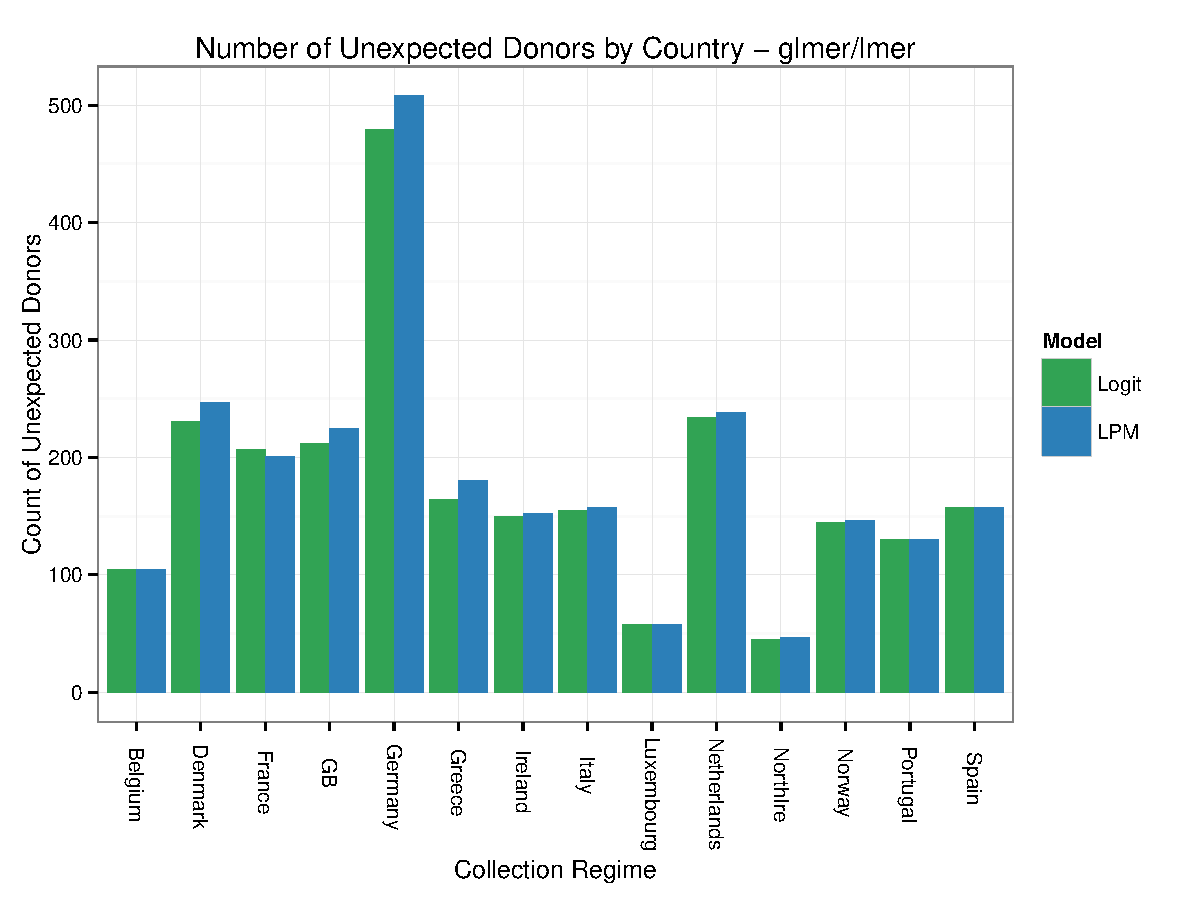
\includegraphics[width=6in]{figures/unexpcount.pdf}
\caption{Number of Unexpected Donors by Country - glmer/lmer\label{fig:countries}}
\end{figure}

\begin{figure}[h]
\centering
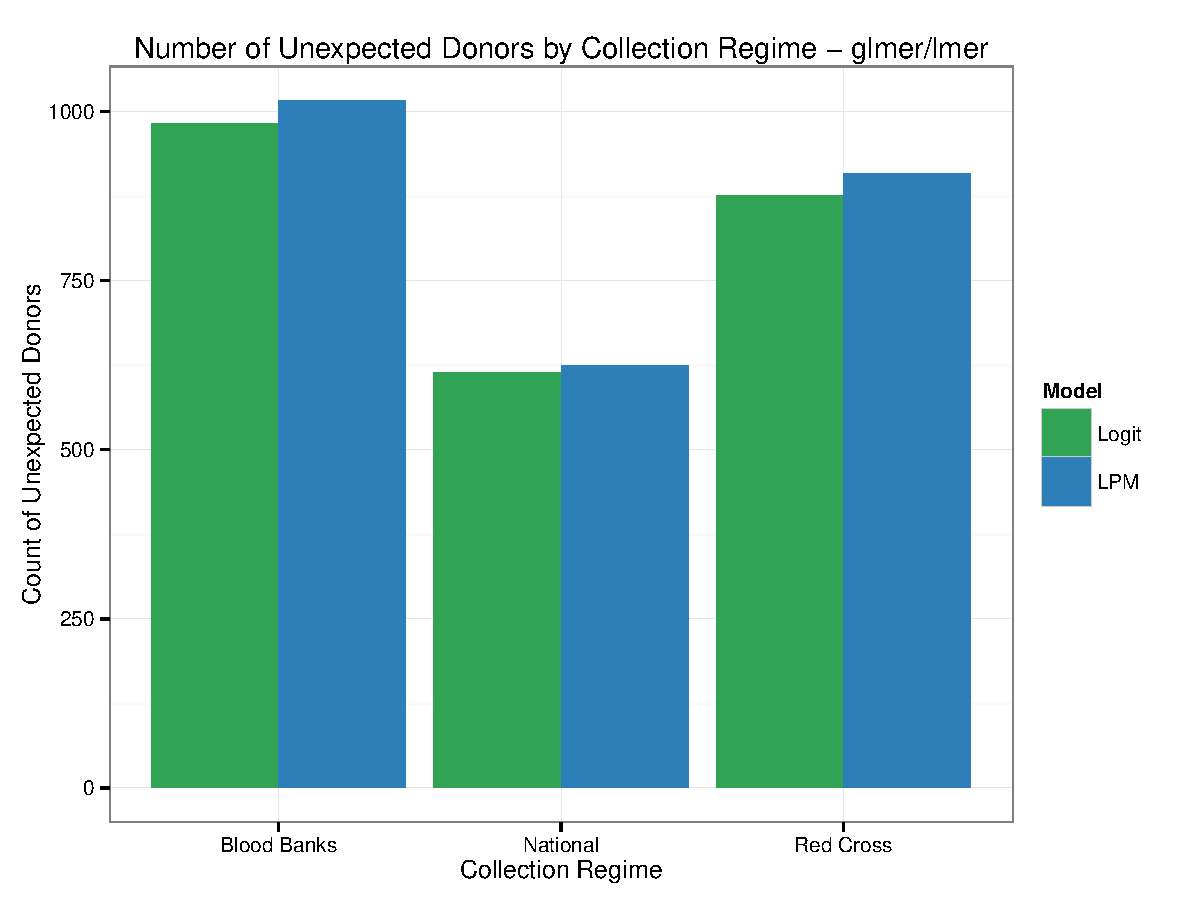
\includegraphics[width=6in]{figures/unexpcr.pdf}
\caption{Number of Unexpected Donors by Collection Regime - glmer/lmer\label{fig:colreg}}
\end{figure}

\newgeometry{margin=1in}
\begin{landscape}
\begin{figure}[h]
\caption{Bootstrap Plot for glmer coefficients \label{fig:boot1plot}}
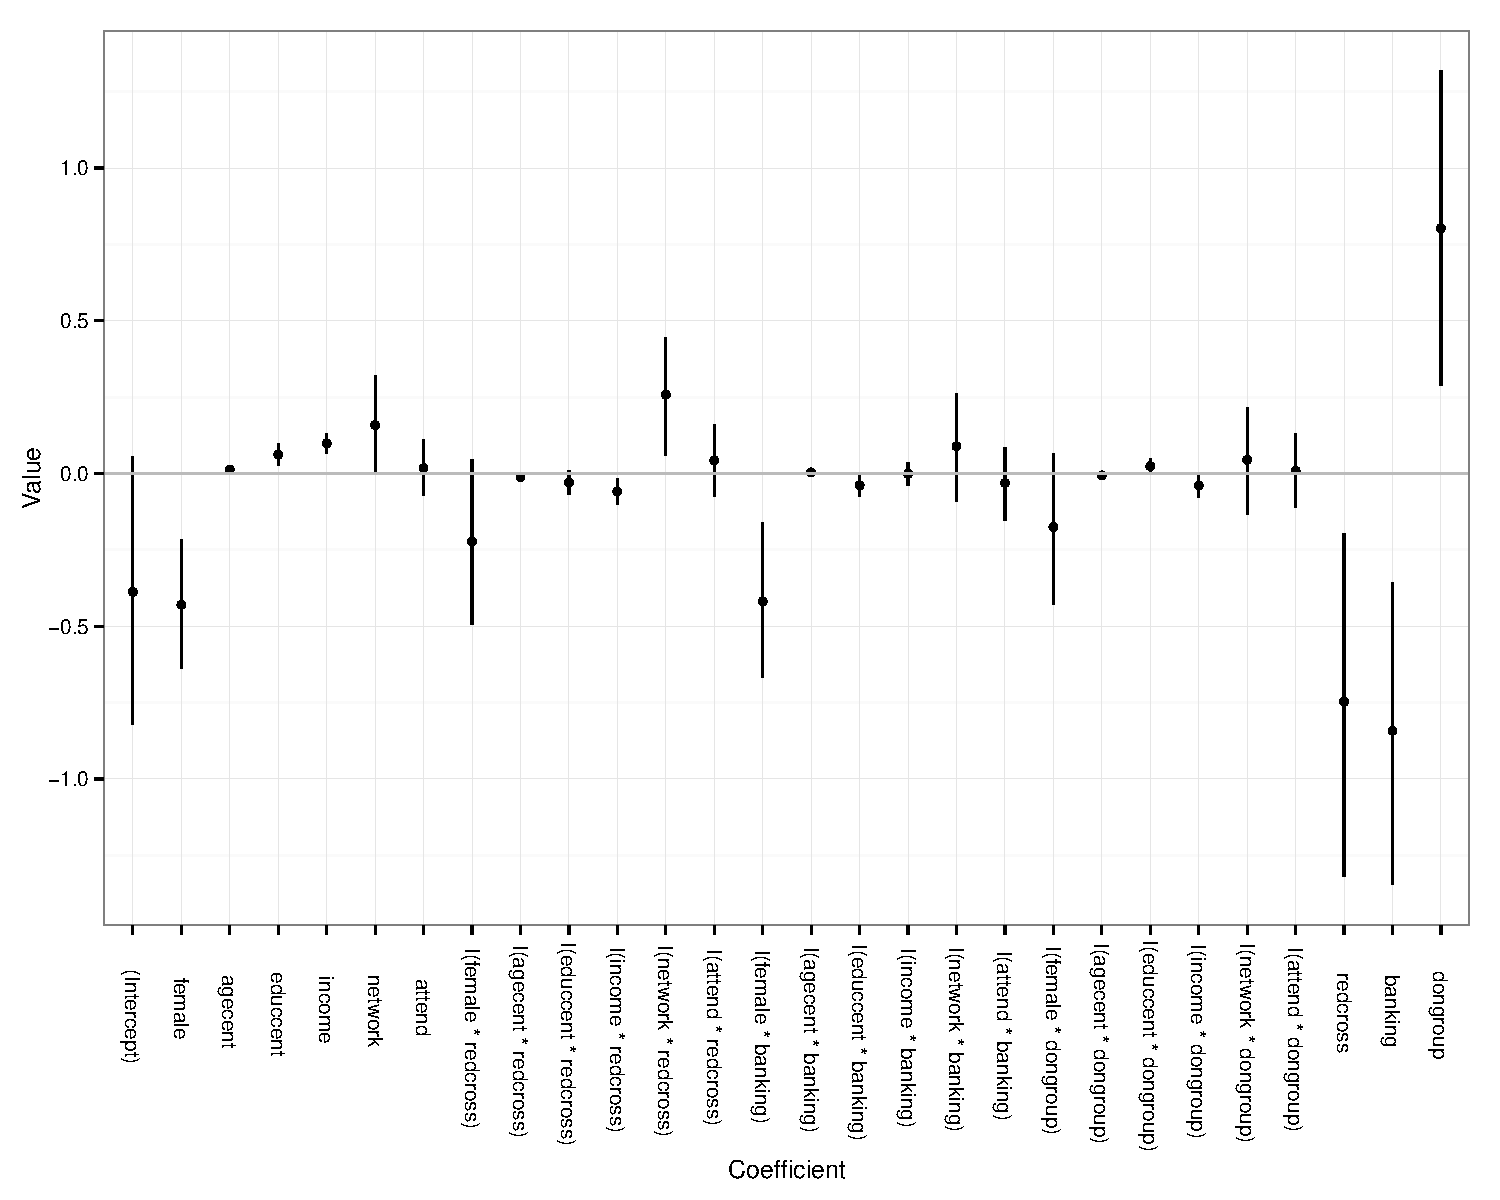
\includegraphics[width=8in]{figures/boot1plot.pdf}
\end{figure}
\end{landscape}
\restoregeometry

\newgeometry{margin=1in}
\begin{landscape}
\begin{figure}[h]
\caption{Bootstrap Plot for lmer coefficients \label{fig:boot2plot}}
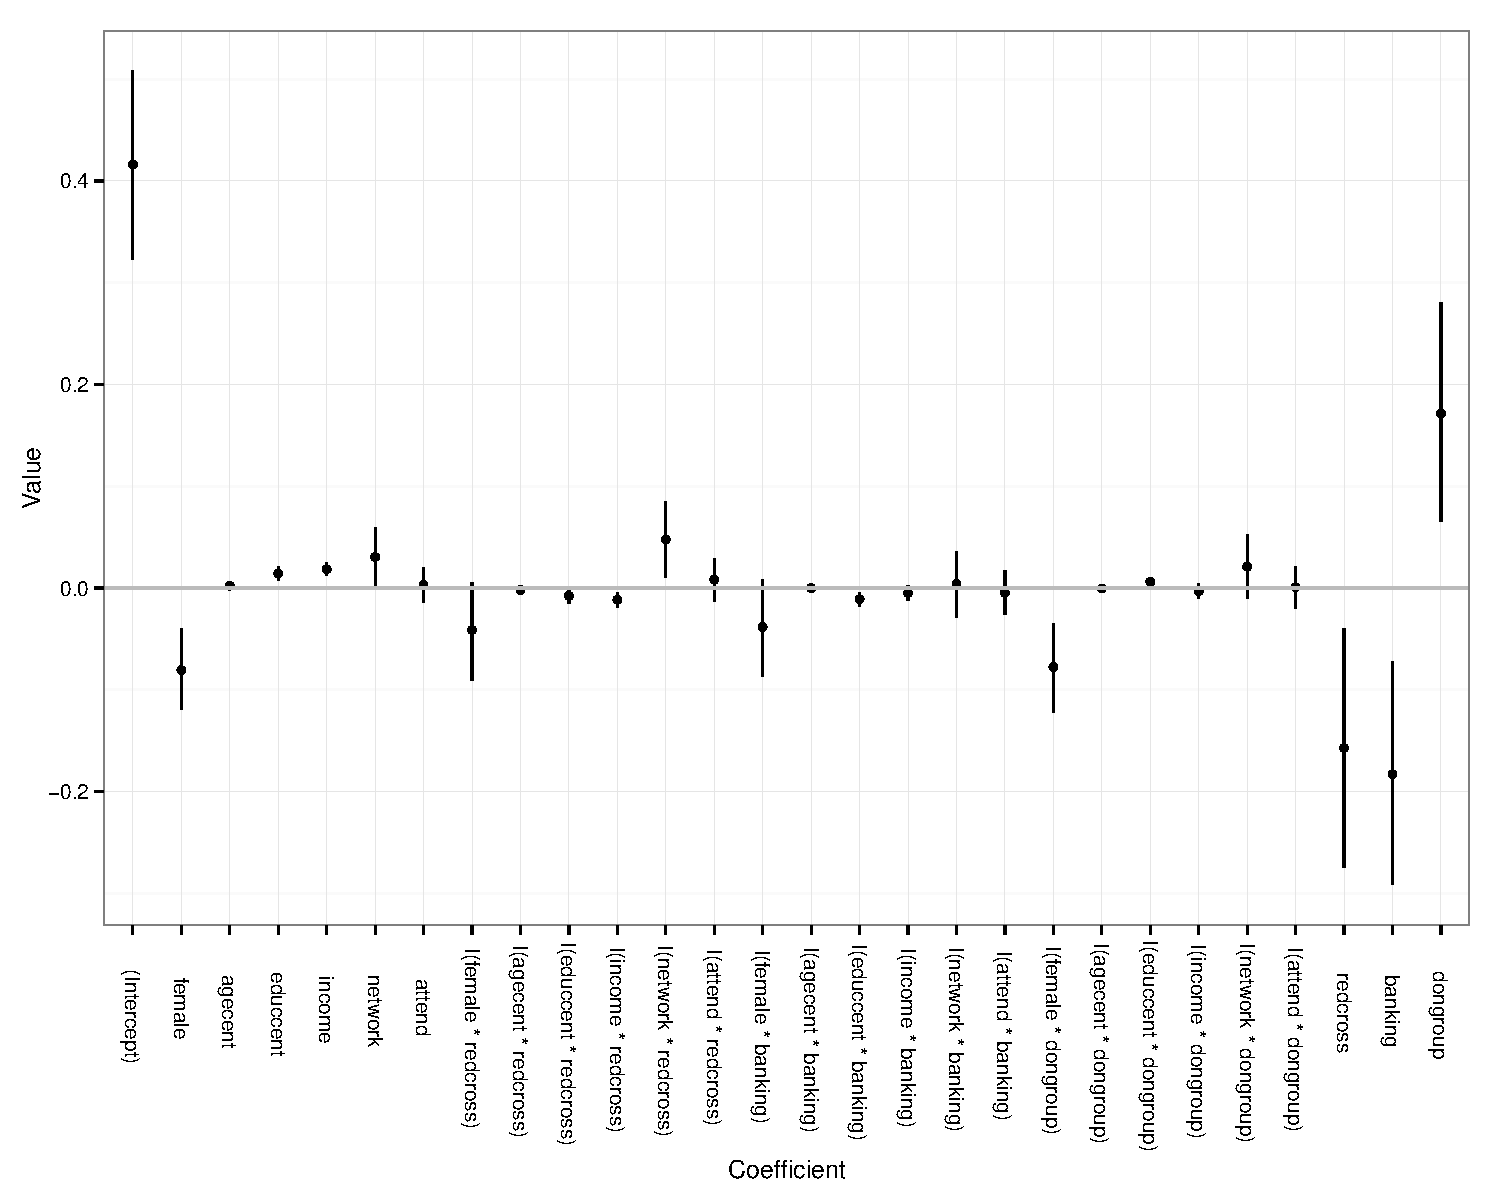
\includegraphics[width=8in]{figures/boot2plot.pdf}
\end{figure}
\end{landscape}
\restoregeometry

\newgeometry{margin=1in}
\begin{landscape}
\begin{figure}[h]
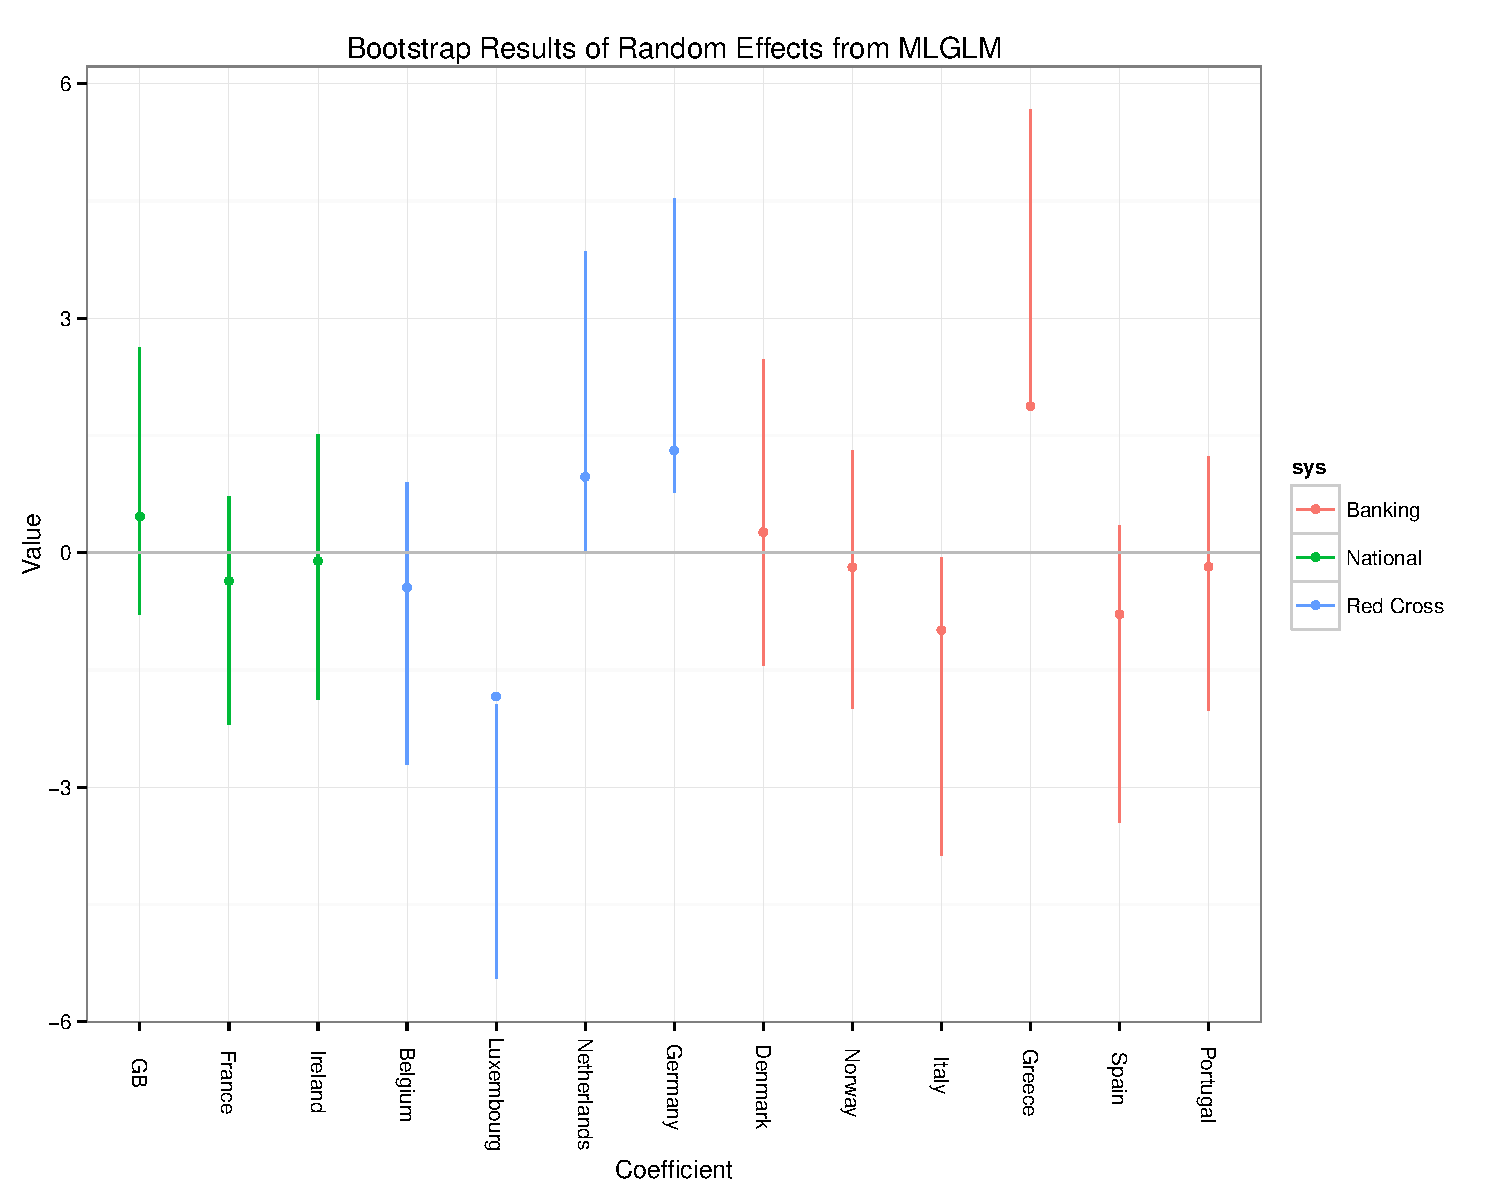
\includegraphics[width=8in]{figures/mlglmrebootplot.pdf}
\end{figure}
\end{landscape}
\restoregeometry

\newgeometry{margin=1in}
\begin{landscape}
\begin{figure}[h]
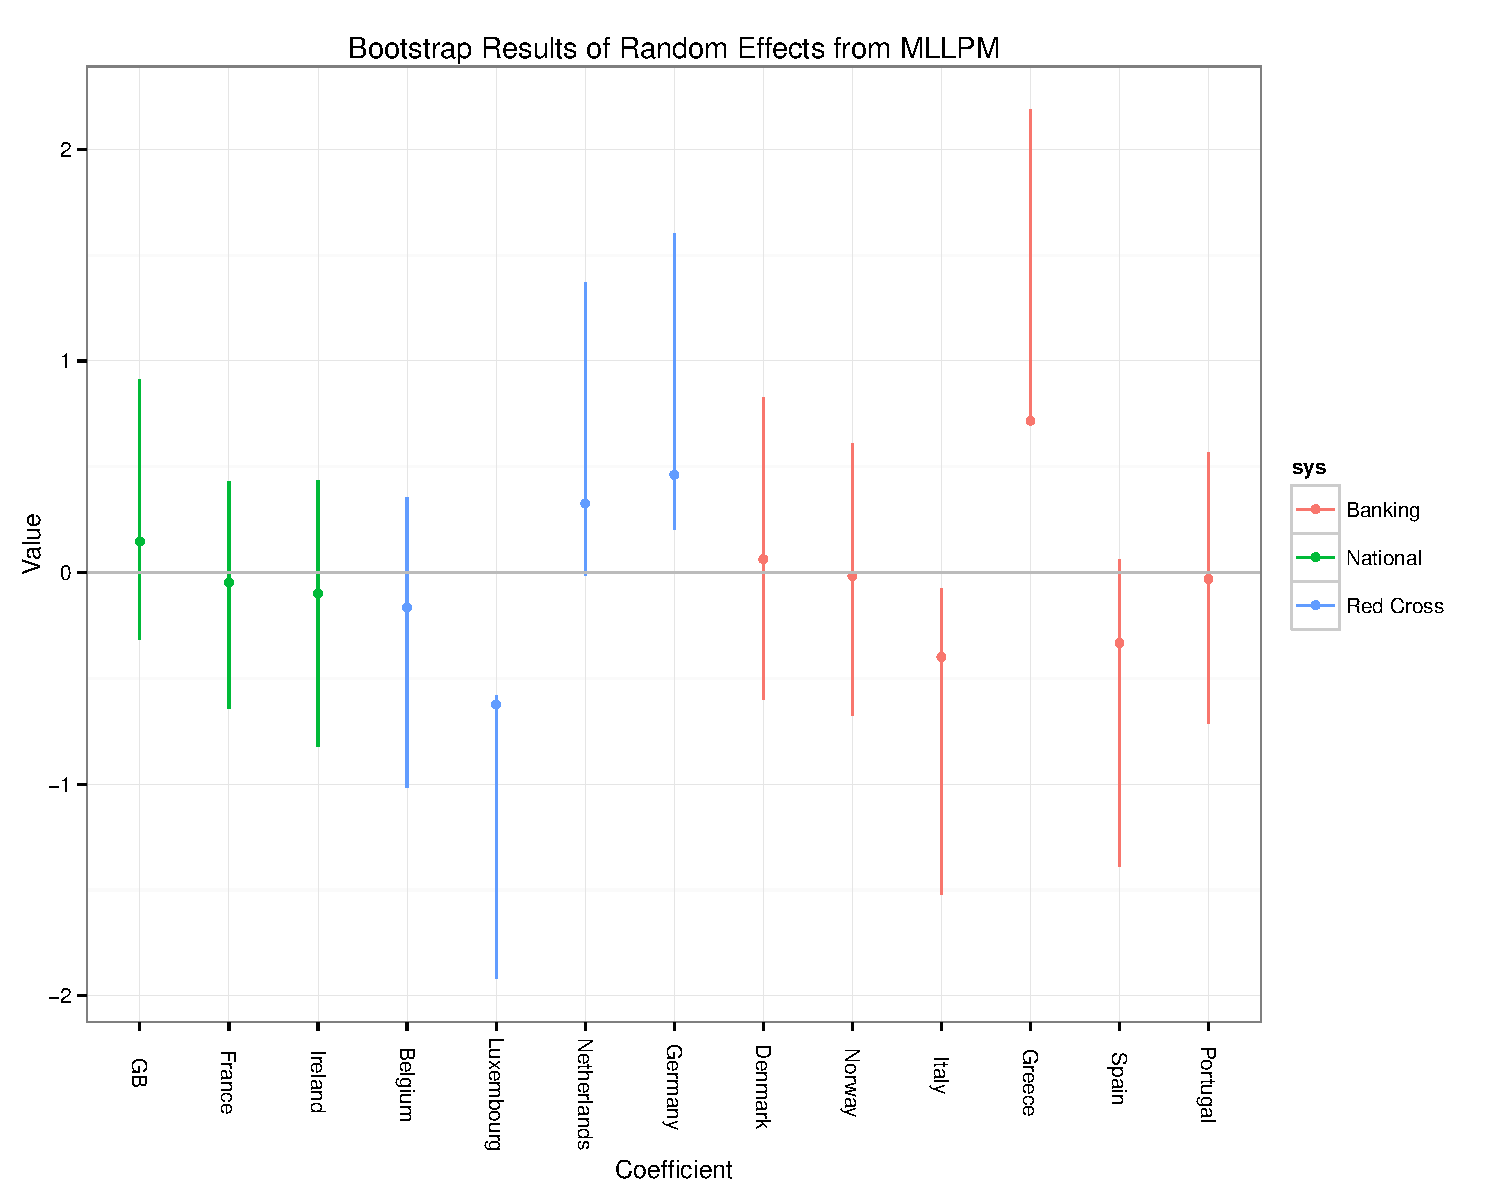
\includegraphics[width=8in]{figures/mllpmrebootplot.pdf}
\end{figure}
\end{landscape}
\restoregeometry

\clearpage

\section{References}\label{references}

\setlength{\parindent}{-0.2in} \setlength{\leftskip}{0.2in}
\setlength{\parskip}{8pt} \vspace*{-0.2in} \noindent

Healy, Kieran. 2000. ''Embedded Altruism: Blood Collection Regimes and
the European Union's Donor Population.'' \emph{American Journal of
Sociology} 105(6):1633--57.

Healy, Kieran. 2003. ''Corrected Tables for 'Embedded Altruism: Blood
Collection Regimes and the European Union's Donor Population'.'' http://kieranhealy.org/files/papers/EA-corrected-tables.pdf


\end{document}